% \chapter{Experimental Simulations and Measurements} \label{ch:distance}
% This chapter describes how distance between finite diploid population and infinite population is calculated.
% Then it discusses simplifications in computations made by our evolutionary equations and in distance computation. 
% And it goes on to discuss results from simulations and convergence of finite diploid population short-term behavior 
% to evolutionary behavior predicted by infinite population model.

\section{Distance}
Let vector ${\bm f}$ represent a finite diploid population; component
${\bm f}_\alpha$ is the prevalence of diploid $\alpha$.  Let the
support $S_{\bm f}$ of ${\bm f}$ be the set of diploids occurring in
the population represented by ${\bm f}$,\\[-0.03in]
\[
S_{\bm f} \; = \; \{ \alpha \, | \, {\bm f}_\alpha > 0 \}
\]
Let ${\bm q}$ similarly represent an infinite diploid population (see
section \ref{Model}).  As points in $\mathbb{R}^{2^\ell
  \times 2^\ell}$, the Euclidean distance between ${\bm f}$ and ${\bm
  q}$ is \\[-0.175in]
\[
\|{\bm f} - {\bm q} \hspace{0.005in} \| \; = \;
  {\sum_{\alpha}}^{\frac{1}{2}} ({\bm f}_\alpha-{\bm q}_\alpha)^2\\[-.02in]
\]
Whereas a naive computation of this distance involves ${2^\ell \cdot
  2^\ell}$ terms, leveraging equation (\ref{model1}) can significantly
reduce the number of terms involved.  Note that
\begin{equation} \label{d1}
\|{\bm f} - {\bm q} \hspace{0.005in} \|^2 \; = \;
\sum_{\alpha \notin {S_{\bm f}}} ({\bm f}_\alpha-{\bm q}_\alpha)^2 +
\sum_{\alpha \in {S_{\bm f}}} ({\bm f}_\alpha-{\bm q}_\alpha)^2 \\[-.02in]
\end{equation}
Using equation (\ref{model1}) --- ${\bm q}_\alpha = {\bm p}_{\alpha_0}
\nudge {\bm p}_{\alpha_1}$ (suppressing superscripts to streamline
notation) --- together with the fact that ${\bm f}_\alpha = 0$ in
every term of the first sum above, the first sum reduces to
\begin{eqnarray}
  \sum_{\langle \alpha_0, \nudge \alpha_1 \rangle \nudge \notin
    {S_{\bm f}}} ({\bm p}_{\alpha_0} \nudge {\bm p}_{\alpha_1})^2 & =
  & \sum_{\langle \alpha_0, \nudge \alpha_1 \rangle} ({\bm
    p}_{\alpha_0})^2 \nudge ({\bm p}_{\alpha_1})^2 \, - \sum_{\langle
    \alpha_0, \nudge \alpha_1 \rangle\in {S_{\bm f}}} \big( {\bm
    p}_{\alpha_0}\nudge {\bm p}_{\alpha_1} \big)^2 \nonumber
  \\[0.05in] & = & {\sum_{g}}^2 ({\bm p}_{g})^2 \, - \sum_{\alpha \in
    {S_{\bm f}}} ( {\bm q}_{\alpha})^2
      \label{d2}
\end{eqnarray}
\mbox{ }\\[-.15in]
It follows from (\ref{d1}) and (\ref{d2}) that
\begin{eqnarray}
  \|{\bm f} - {\bm q} \hspace{0.005in} \|^2
  & = & 
      {\sum_{g}}^2 ({\bm p}_{g})^2 \, +
      \sum_{\alpha \in {S_{\bm f}}} ({\bm f}_\alpha-{\bm q}_\alpha)^2 -
      \sum_{\alpha \in {S_{\bm f}}} ( {\bm q}_{\alpha})^2
      \nonumber \\[0.05in]
      & = &
      {\sum_{g}}^2 ({\bm p}_{g})^2 \, +
      \sum_{\alpha \in {S_{\bm f}}} {\bm f}_\alpha ({\bm f}_\alpha- 2 {\bm q}_\alpha) \label{d3}
\end{eqnarray}
\mbox{ }\\[-.1in] which involves $2^\ell + |S_{\bm f}|$ terms,
assuming that  $S_{\bm f}$ is known as a byproduct of computing ${\bm f}$.

(\ref{d3}) computes distance between finite and infinite population efficiently.


\section{Simplification} 
The haploid case simplified by equations (\ref{Mhat}) and (\ref{model5})
are the consequence of specializing to Vose's infinite population model and computing in the Walsh basis. Time switching between the standard basis and the Walsh basis is negligible; the fast Walsh transform (in dimension $n$) has complexity $n \nudge \log n$ \cite{Shanks1969}.

Only one mixing matrix as opposed to $2^\ell$ matrices is needed to compute the next generation; evolution equation (\ref{model5}) references the same matrix for every $g$, whereas evolution equation (\ref{model3}) depends upon a different matrix $M_g$ for each choice of $g$. The matrix is computed by a single sum as opposed to a triple sum; compare equation (\ref{Mhat}) with equation (\ref{transmission}).  Also, the relevant quadratic form is computed with a single sum as opposed to a double sum; computing via (\ref{model5}) is linear time in the size of $g \mathcal{R}$ (for each $g$) as opposed to the quadratic time computation (for each $g$) represented by equation (\ref{model3}).

From a computational standpoint, the best-case scenario is where
recomputation of the matrices mentioned in the previous paragraph is
obviated by sufficient memory.  The reduction from $2^\ell$ matrices
to one matrix helps significantly in that regard. To demonstrate this
advantage in concrete terms, consider genomes of length $\ell = 14$.
Using $2^{14}$ matrices each of which contains $2^{14} \times \nudge
2^{14}$ entries of type \verb@double@ requires $32$ terabytes, whereas
the mixing matrix at $2$ gigabytes fits easily within the memory of a
laptop.  Moreover, for a population size of $N \le 2^{20}$, the
distance computation described in the previous section reduces the
number of terms involved by a factor of
$2^{28}/(2^{14} + 2^{N}) \; > \; 252$.

\section{Convergence}

This section presents a cursory numerical investigation of the
convergence of finite diploid population short-term behaviour to that
of the infinite diploid population model as described in section 2
(the underlying haploid model for the infinite population case is
described in section \ref{Model}).

Equations (\ref{model1}), (\ref{Mhat}),
(\ref{model5}), (\ref{d3}) were employed to illustrate efficient
computation of the distance
\[
d \; = \; \|{\bm f}^n - {\bm q}^n \nudge \|
\]
where ${\bm f}^n$ and ${\bm q}^n$ represent finite and infinite diploid
populations at generation $n \in \{1,2,4,8,16,32,64,128\}$
respectively, beginning from a random initial population (${\bm f}^0 =
{\bm q}^0$). Genome lengths $\ell \in \{4,6,8,10,12,14\}$ and population
sizes $N = 2^i$ for integer $0 \le i \le 20$ were considered.  The
crossover distribution ${\bm \chi}$ corresponds to independent assortment of
bits, and the mutation distribution ${\bm \mu}$ corresponds to independent
bit mutation probability $0.001$,

\[
{\bm \chi}_m \; = \; 2^{-\ell}, \;\;\;\;\; {\bm \mu}_g \; = \; (0.001)^{{\bf 1}^{\rm T}
  g}(0.999)^{\ell - {\bf 1}^{\rm T} g}
\]
(subscripts above on the left hand side of an equality are interpreted
on the right hand side of the equality as column vectors in
$\mathbb{R}^{\ell}$). The finite population case is computed using the
itemized procedural definition given in section \ref{Model}; the transmission
function (\ref{transmission}) corresponds to ${\bm \mu}$ and ${\bm
  \chi}$ above (bits mutate independently and are freely assorted).

\begin{figure}[H]
\begin{center}
\subfloat[$\ell = 4$.]{
\resizebox*{6.5cm}{!}{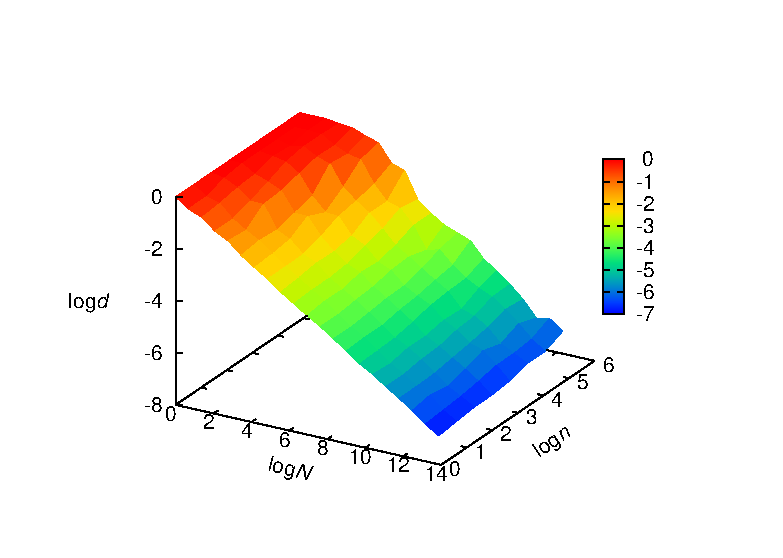
\includegraphics{figures/eps/surf/b4.eps}}}\hspace{5pt}
\subfloat[$\ell = 6$.]{
\resizebox*{6.5cm}{!}{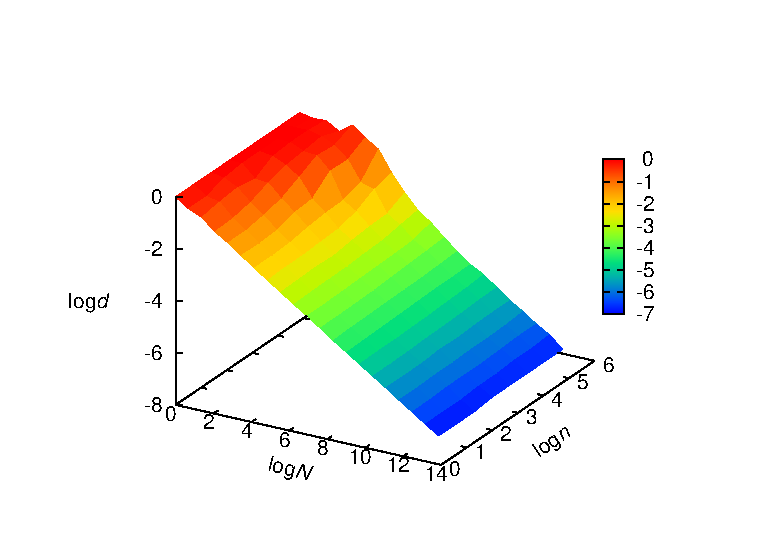
\includegraphics{figures/eps/surf/b6.eps}}}
\end{center}
  
\begin{center}
\subfloat[$\ell = 8$.]{
\resizebox*{6.5cm}{!}{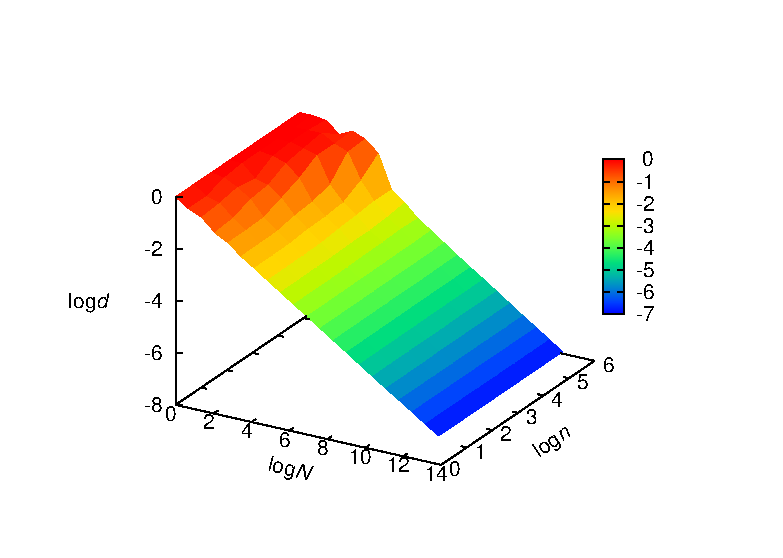
\includegraphics{figures/eps/surf/b8.eps}}}\hspace{5pt}
\subfloat[$\ell = 10$.]{
\resizebox*{6.5cm}{!}{\includegraphics{figures/eps/surf/b10.eps}}}
\end{center}

\begin{center}
\subfloat[$\ell = 12$.]{
\resizebox*{6.5cm}{!}{\includegraphics{figures/eps/surf/b12.eps}}}\hspace{5pt}
\subfloat[$\ell = 14$.]{
\resizebox*{6.5cm}{!}{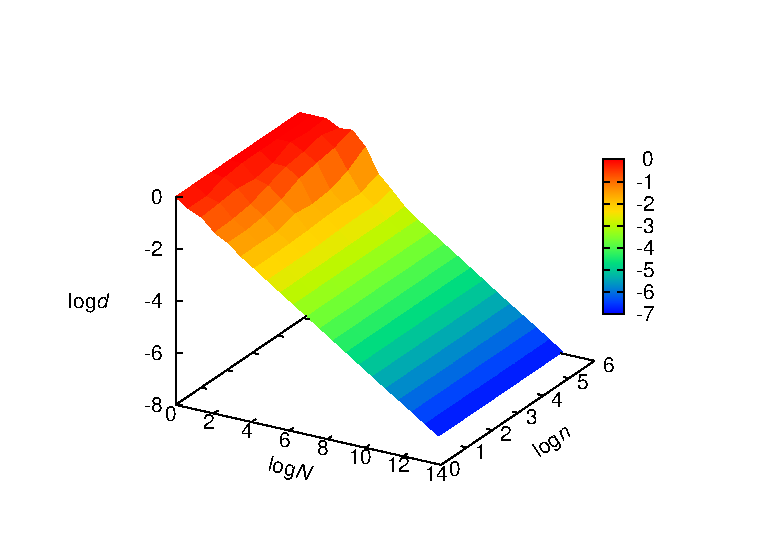
\includegraphics{figures/eps/surf/b14.eps}}}
\caption{\textbf{Convergence of finite population behaviour:} $d$ is
  distance between finite population ${\bm f}^n$ and infinite
  population ${\bm q}^n$ at generation $n$, population size $N$, for
  genome length $\ell$ (bits).}
\label{convergence}
\end{center}
\end{figure}

The data, presented in six surface graphs above and organized by
genome length, shows a near linear dependence of $\log d$ on $\log N$.
As expected, the graphs show smoothing with increasing genome length
(the computation of $d$ involves averaging over $\ell$ components),
and also with increased population size (as explained in
\cite{Vose1999}, the initial transient of a finite haploid population
trajectory converges as $N \rightarrow \infty$ to the corresponding
infinite population model).

%\newpage
  Of particular interest is the linear trend exhibited above.  The
  slope $m$ and intercept $b$ of the regression line
  \begin{equation} \label{regresion}
  \log d = m \log N + b
  \end{equation}
was computed using the data above; each was plotted against genome
length $\ell$ and organized by generation $n$. The resulting
graphs are displayed below.

\begin{figure}[H]
\begin{center}
\subfloat[Slope $m$, genome length $\ell$.]{
\resizebox*{7cm}{!}{\includegraphics{figures/eps/slope/m.eps}}}\hspace{5pt}
\subfloat[Intercept $b$, genome length $\ell$.]{
\resizebox*{7cm}{!}{\includegraphics{figures/eps/slope/b.eps}}}
\caption{\textbf{Regression parameters:} multi-plot of slope $m$ and intercept $b$ for generation  $n \in \{1,  2,  4,  8,  16,  32,  64,  128\}$ .}
\label{regression-parameters}
\end{center}
\end{figure}

Taking the exponential of the regression line (\ref{regresion}) yields
the estimate
$d \approx N^m e^b $.

Slopes of the regression lines shown in {\bf Figure \ref{regression-parameters}} are
approximately $-0.5$, indicating
\begin{equation}
\label{covergenceDistance}
d \; \approx \; k/\sqrt{N}.
\end{equation} 
Equation \ref{covergenceDistance} agrees with  equation \ref{convergenceRHS} which shows the expected rate of convergence for the single-step haploid case; the distance is inversely proportional to square root of population size.

The consistent convergence rate
across multiple generations is somewhat surprising, simulation
results above indicate it may persist to generation $n = 128$.

The intercept graphs above show the constant of proportionality $k =
e^b$ decreases monotonically with genome length $\ell$, and increases
monotonically with generation $n$.  The increase in $k$ for larger $n$
seems to be a manifestation of the growing nonlinearity uniformly
exhibited by the plots in {\bf Figure \ref{convergence}} as $n$ increases.  It seems
likely that the nonlinearity results from genetic drift experienced by
finite populations (see \cite{CrowKimura}).


